\documentclass[12pt, a4paper]{article}
\usepackage[a4paper, bindingoffset=0.2in, %
left=0.5in,right=0.5in,top=0.5in,bottom=0.5in,%
footskip=.25in]{geometry}
\usepackage{graphicx}
\usepackage{amssymb}
\usepackage{amsmath}
\usepackage{hyperref}
\usepackage{physics}

\title{Final Exam Report}
\author{Ali Abolhassanzadeh Mahani \\ 97110863}
\date{}

\begin{document}
	\maketitle
	\section{Problem 1}
	\subsection{Introduction}
	I made the \texttt{BlumeCapel} class with init function that takes values of J, D, and length L, and  creates a system with random spins with 
	side length $L$. In each \texttt{metropolis()} time step, the system gives all of the cells (ammortized) a chance to change spin. since we have
	2 options to change to, we take one randomly and then use the metropolis \texttt{decision()}  method to see if we will change the spin. For the 
	system to reach equilibrium, I devised a method called \texttt{eqaulize()} that evolves the system 20 time steps in each iteration, and saves
	the energy of the system. Then, it finds the auto-correlation of the energies and if the it's lower than a threshold, the system is equalized. 
	
	I made the \texttt{get\_data()} method, to take data from the equalized system in each \texttt{step} time steps. I also made the 
	\texttt{simulate()} method, that simulated the system to various values of J and D and returns the collected data. I then save the data to
	a \texttt{.npy} file in the \texttt{data/} subdirectory and use the \texttt{analysis.py} file to draw the plats.
	
	\subsection{Part A}
	I plotted the change in each variable, over various D, for different values of J. (Fig~\ref{fig:chi_10}, ~\ref{fig:n3_10}, ~\ref{fig:mag_10})
	
	\begin{figure}[h!]
		\centering
		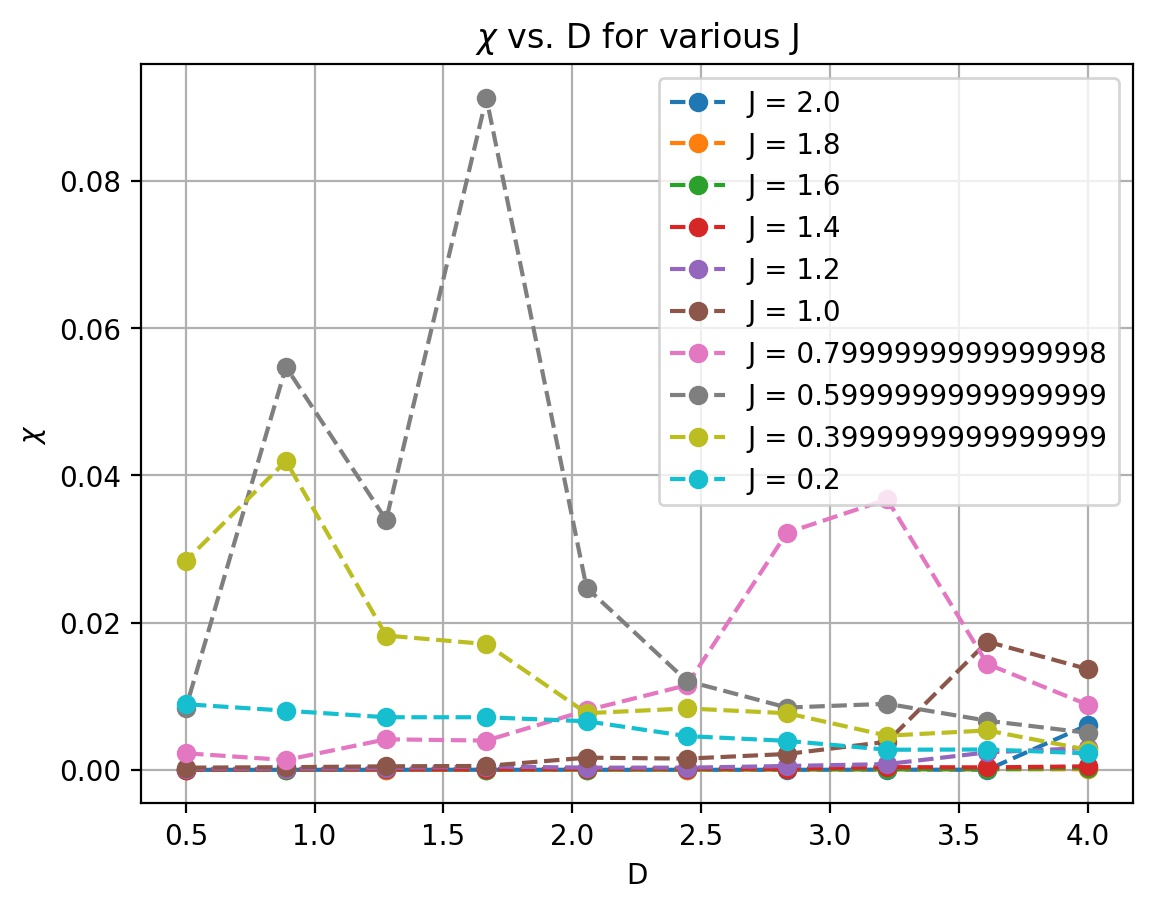
\includegraphics[width=.8\linewidth]{../p1/results/chi_10.jpg}
		\caption{We can see that the critical value of D changes with J}
		\label{fig:chi_10}
	\end{figure}

	\begin{figure}[h!]
	\centering
	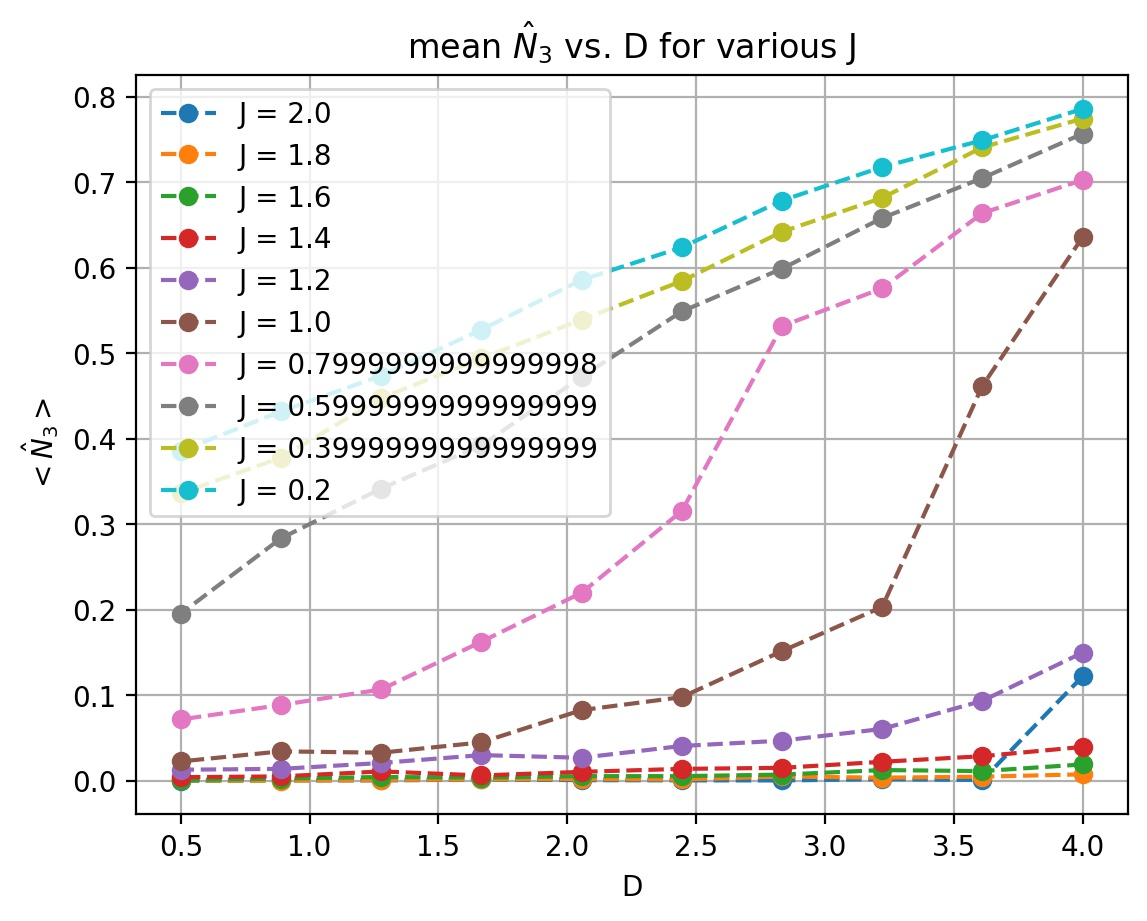
\includegraphics[width=.8\linewidth]{../p1/results/mean_n3_10.jpg}
	\caption{We can see that the critical value of D changes with J}
	\label{fig:n3_10}
\end{figure}

	\begin{figure}[h!]
	\centering
	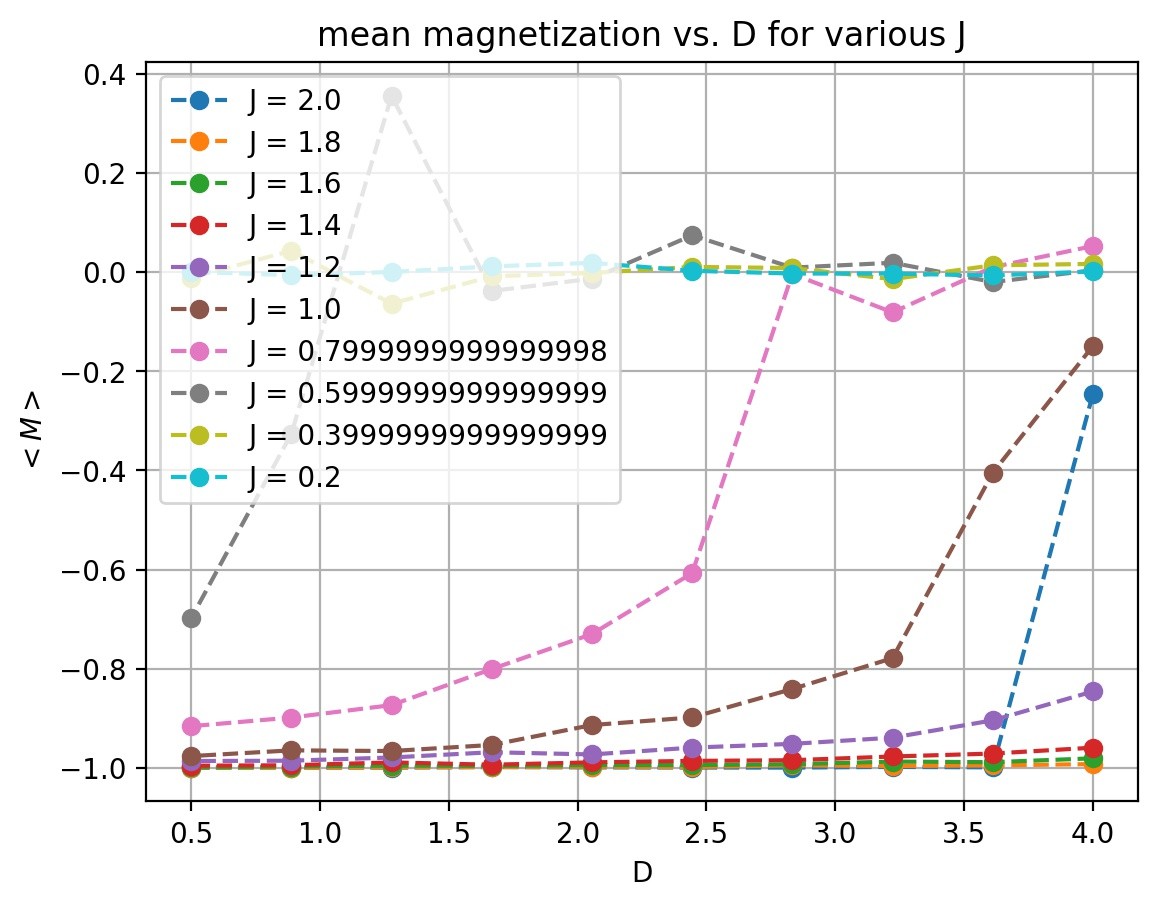
\includegraphics[width=.8\linewidth]{../p1/results/magnetization_10.jpg}
	\caption{We can see that the critical value of D changes with J}
	\label{fig:mag_10}
\end{figure}
	
	\subsection{Part B}
	for $L = \{20, 40\}$, the runtime was too high and couldn't complete the data collection in time.
	\section{Problem 2}
	\subsection{Theory}
	The leonard-Jones potential is as follows:
		\begin{equation}
		U_{ij} = 4\epsilon \left(\left(\frac{\sigma}{r_{ij}}\right)^{12} - 
		\left(\frac{\sigma}{r_{ij}}\right)^6\right), \; 
		r_{ij} \equiv \norm{\vec{r}_i - \vec{r}_j}
		\label{eq:leonard_jones}
	\end{equation}
	
	The reduced units is as follows:
	\begin{equation}
		\begin{aligned}
			E' &= \frac{E}{\epsilon}, \\
			L' &= \frac{L}{\sigma}, \text{L = length},\\
			 m' &= \frac{m}{m_{arg}}, \\
			T' &= k_B T
		\end{aligned}
	\end{equation}
	
	The values for the constanst is as follows:
	\begin{equation}
		\begin{aligned}
			\epsilon &\simeq 15.03 \times 10^{-22} J,\\
			\sigma &\simeq 3.419 \times 10^{-10} m,\\
			m_{arg} &\simeq 6.63 \times 10^{-26} kg\\
			k_B &\simeq 1.38 \times 10^{-23} \frac{J}{K}
		\end{aligned}
	\end{equation}

	Now I show the relation for density, perssure, temperature, and time in Table~\ref{tab:reduced}
	
	\begin{table}[h!]
		\centering
		\begin{tabular}{|c|c|c|}
	\hline
\multicolumn{3}{|c|}{$f = \alpha f'$}\\
\hline
 $\alpha$ & param & value \\
 \hline
$\text{density} \;\rho$ & $\frac{m_{arg}}{\sigma^3}$ & $4142.97$\\
 \hline
 $\text{time}\; \tau$ & $\sqrt{\frac{m_{arg} \sigma^2}{\epsilon}}$ & $1.63 \times 10^{-12}$ \\
 \hline
$\text{temp.} \; T$ & $\frac{\epsilon}{k_B}$ & $117.8$\\
 \hline
 $\text{pressure}\; P$ & $\frac{\epsilon}{\sigma^3}$ & $9.94 \times 10^{7}$ \\	
 \hline
		\end{tabular}
	\caption{The coefficients that relate the SI to the reduced unit system. }
	\label{tab:reduced}
	\end{table}
	
	\newpage
	\subsection{Psudocode}
	Choosing $L = 7$ in reduced units gives $\rho = 0.36$ for 128 particles. And having max value of velocities to me $1.5$ gives a temperature of about $80 K$.\\
	
	\noindent\texttt{
	\noindent def \_\_init\_\_():\\
	x, y, z $\leftarrow$ positions // uniformly distributed inside the box\\
	self.L = 7  // size of the box L * L * L\\
	self.volume = self.L ** 3 \\
	self.accel $\leftarrow$ accel() \\ 
	v\_x, v\_y, v\_z = // random velocity with max velocity around 1.5\\ 
	stabilize()\\ \\
	def accel(x, y, z):\\
		// return acceleration for each direction considering periodic boundaries\\ \\
	def stabilize():\\
		// take mean of the velocity of the particles as center of mass velocity\\
		// substract all the velocities by that value\\ \\
	def timestep():\\
		// verlet method to evolve\\
		h = 0.001\\
		x, y, z += v\_x, v\_y, v\_z * h + 0.5 * self.accel * h ** 2 // update position\\
		v\_x, v\_y, v\_z += self.accel * h * 0.5 // update speed partially\\
		self.accel = accel() // update self.accel \\
		v\_x, v\_y, v\_z += self.accel * 0.5 * h //completely update veolcities\\ 
		// set periodic boundary conditions that if a particle moves out, comes in from the other side\\ \\
		def temp():\\
		// take sum of square of velocities and divide by 3 * 127 \\ \\
	}

	There's also a fully functional code for this in \texttt{p2/} directory. The only necessity is to specify the initial velocity and the positions. One can 
	just change the value of \texttt{self.dim} to $3$ and the code is ready to simulate the 3-D version of Argon atoms.

	\section{Problem 4}
	I implemented the \emph{euler} and \emph{backward euler} in the file \texttt{eulers.py}. Then, in \texttt{main.py}, I import them and use them
	to calculate the results. Both methods store and return an array for \texttt{time}, \texttt{x}, \texttt{x\_dot}, and \texttt{count} which is the l
	ength of the previous arrays. 
	
	\subsection{Part A}
	I calculated the curves using \emph{euler} method for the given time steps. The results are in Fig~\ref{fig:euler} blow:
	
	\begin{figure}[h!]
		\centering
		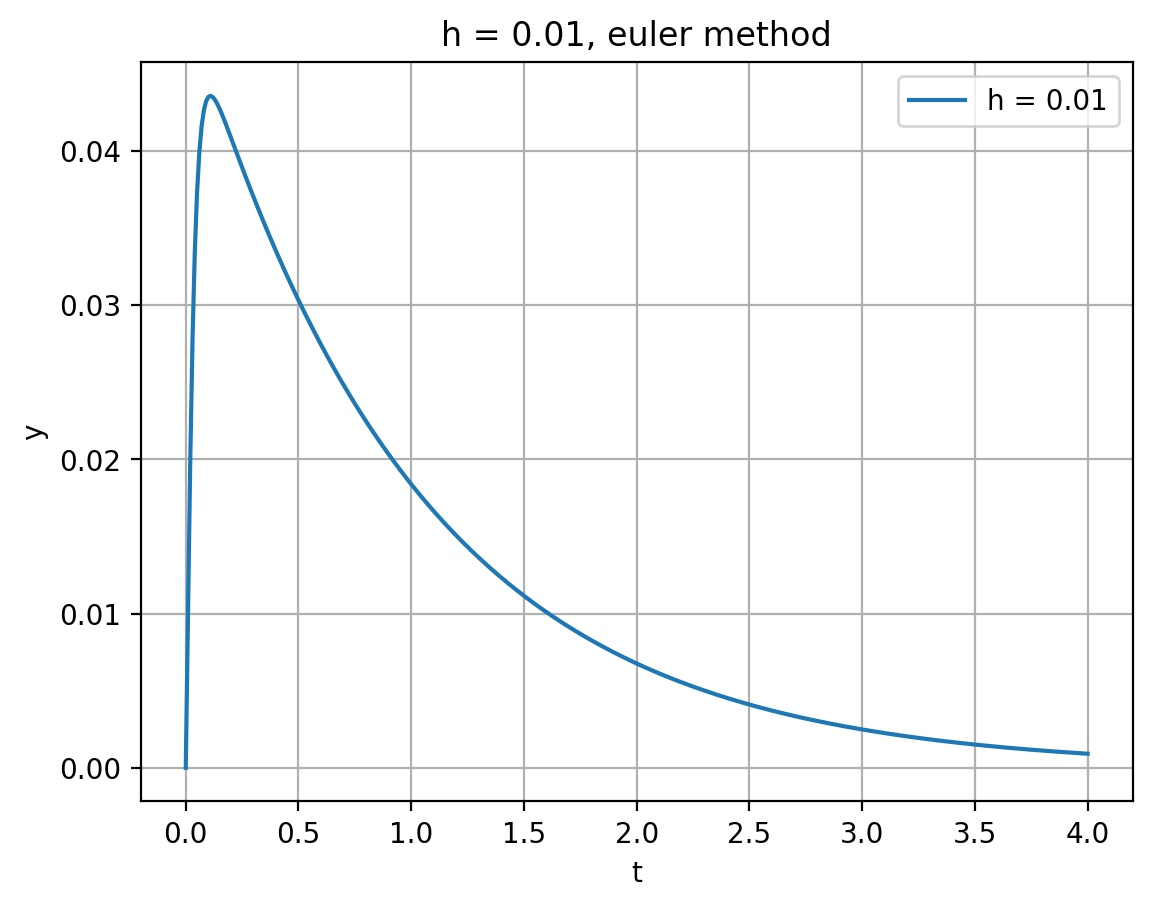
\includegraphics[width=.45\linewidth]{../p4/results/euler_0.01.jpg}
		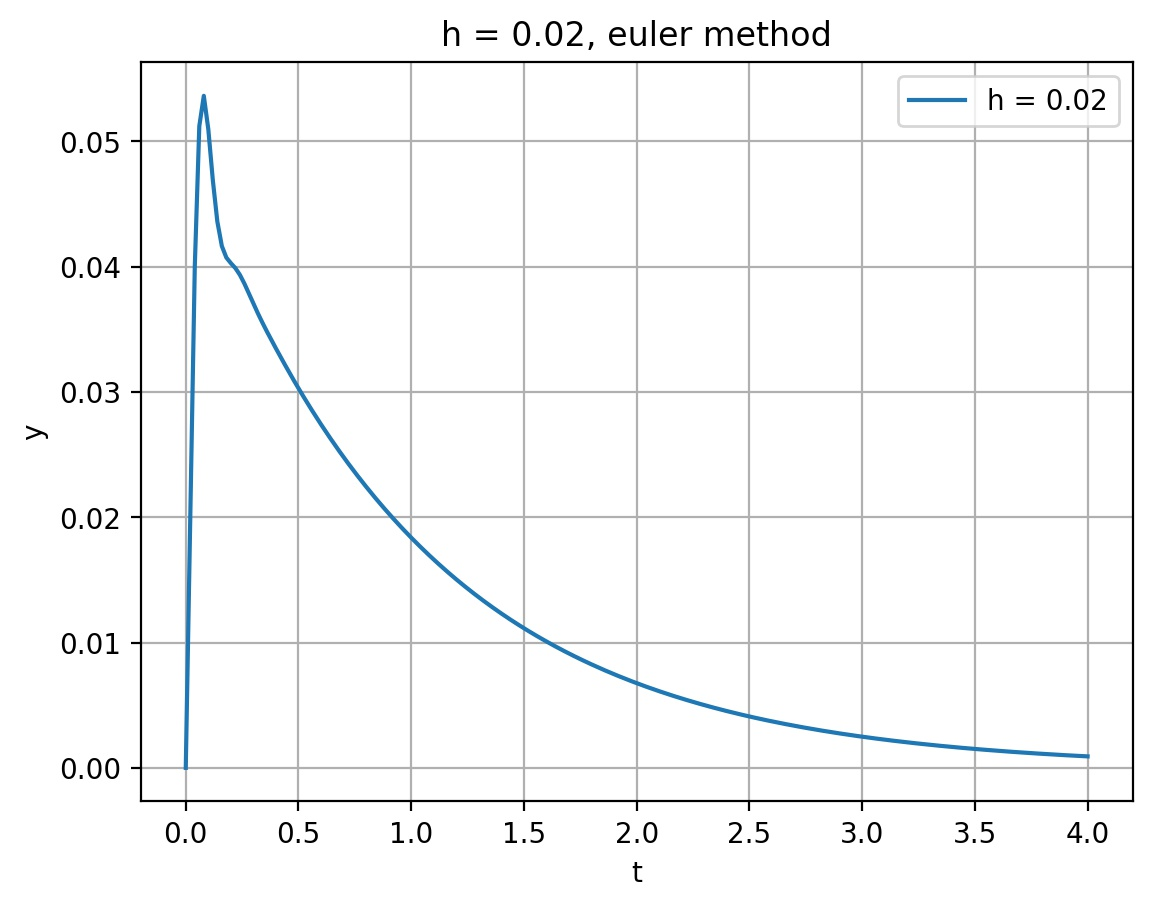
\includegraphics[width=.45\linewidth]{../p4/results/euler_0.02.jpg}
		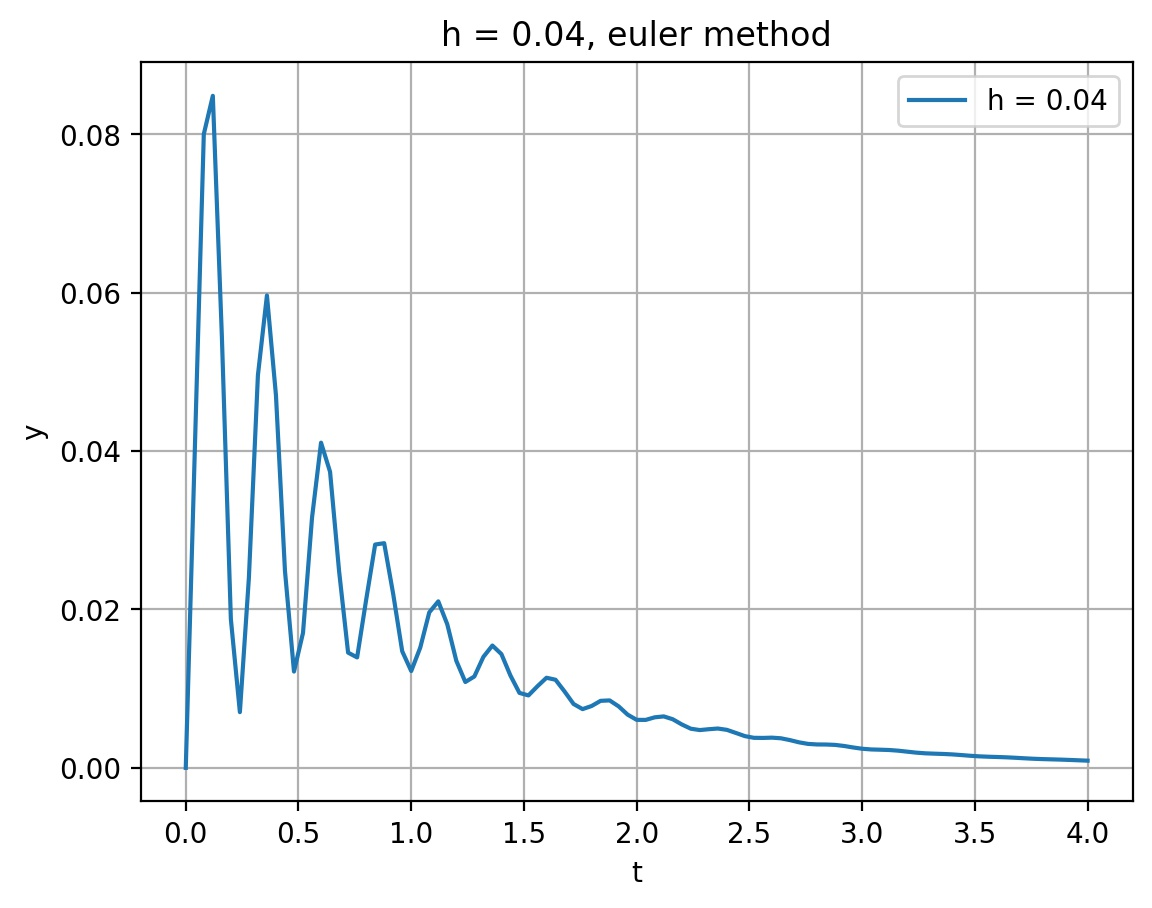
\includegraphics[width=.45\linewidth]{../p4/results/euler_0.04.jpg}
		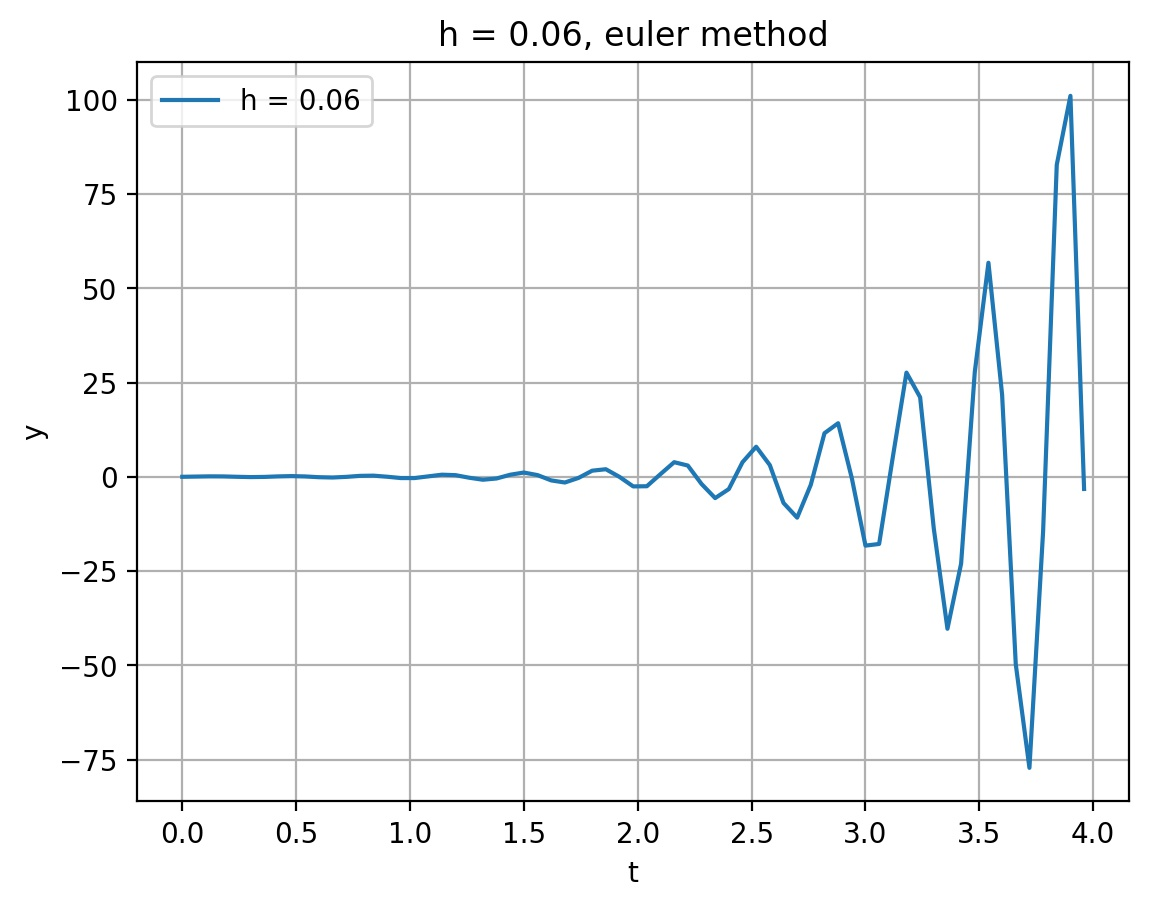
\includegraphics[width=.45\linewidth]{../p4/results/euler_0.06.jpg}
		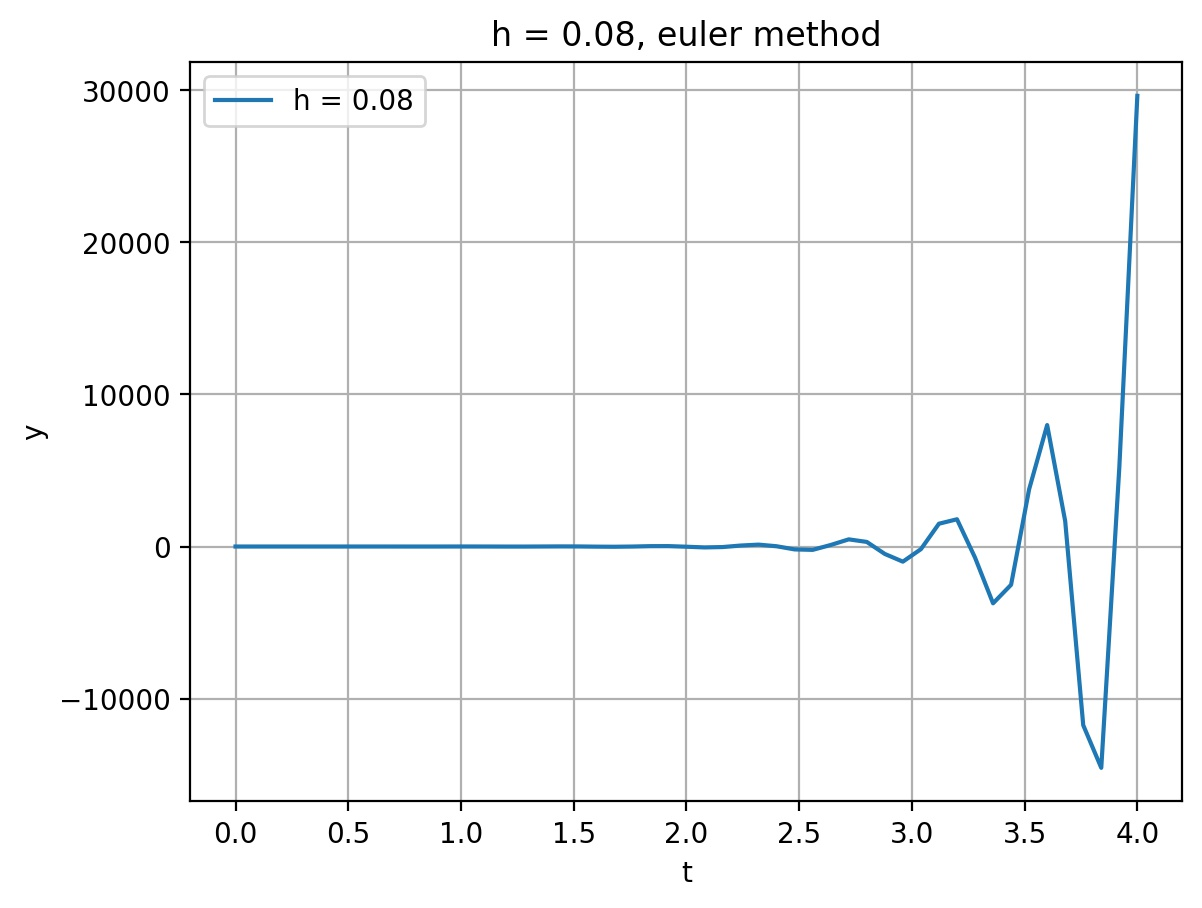
\includegraphics[width=.45\linewidth]{../p4/results/euler_0.08.jpg}
		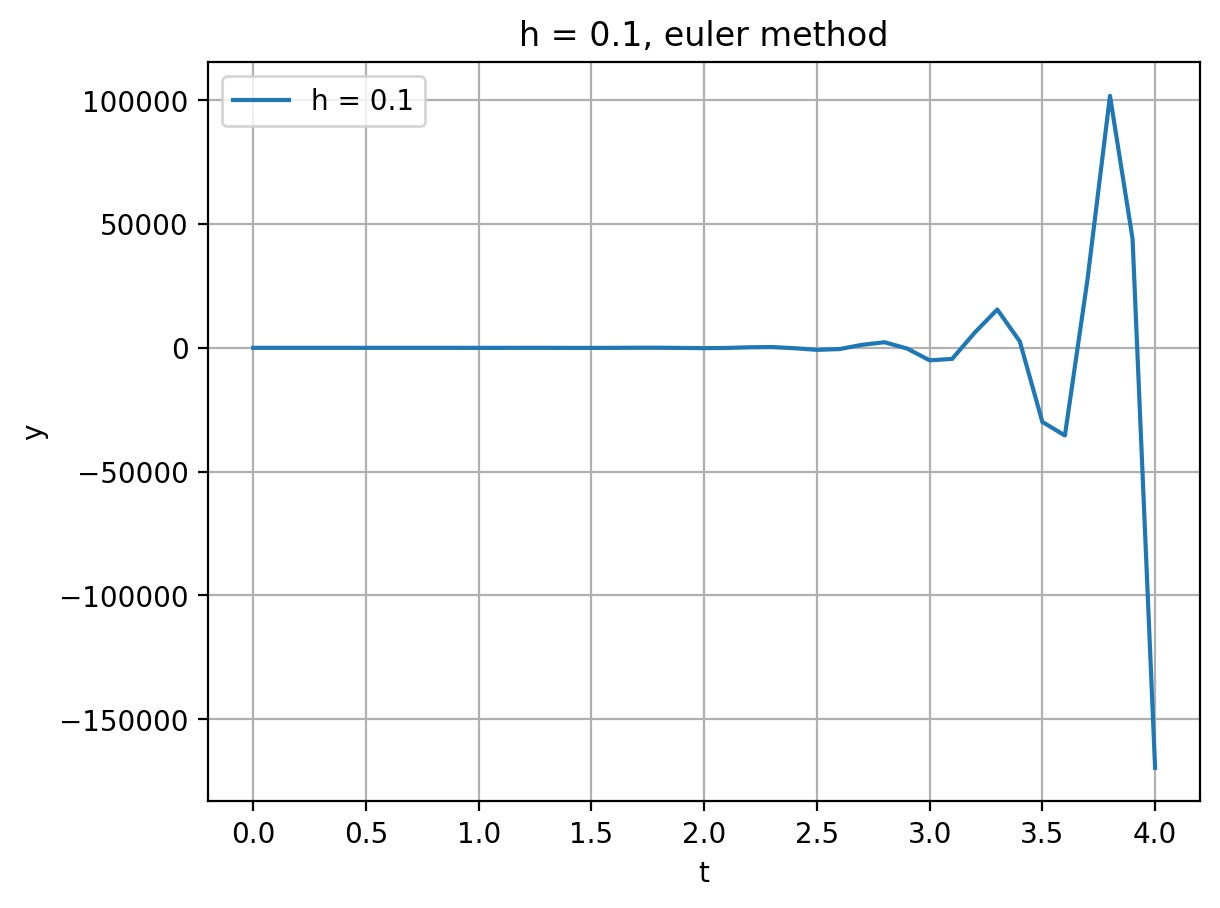
\includegraphics[width=.45\linewidth]{../p4/results/euler_0.1.jpg}
		\caption{The integral curve for various values of $h$ using the euler method. It can be seen that from a value of $h$, the results become 
			\emph{unstable}}
		\label{fig:euler}
	\end{figure}

	\subsection{Part B}
	Did the same as part A using the \emph{backward euler} method. Results in Fig~\ref{fig:backward_euler}
	
	\begin{figure}[h!]
		\centering
		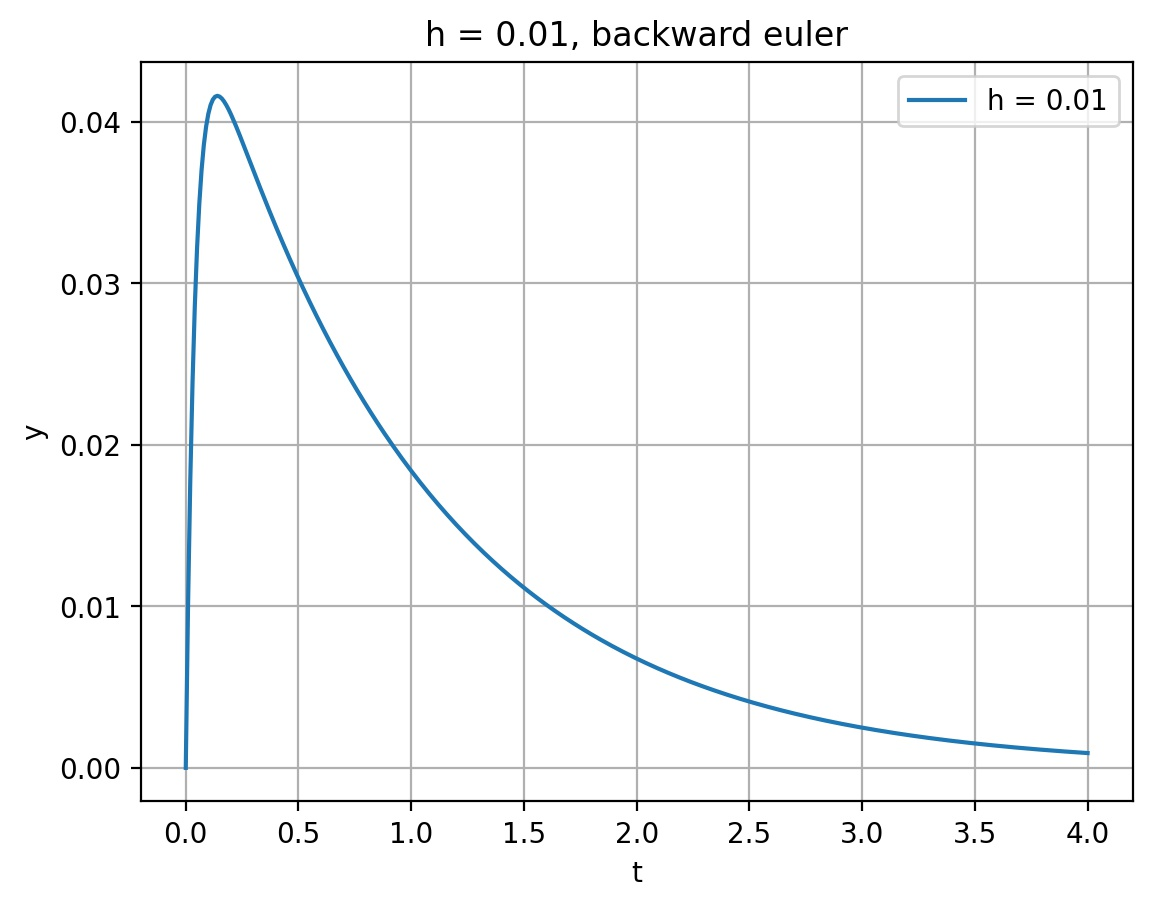
\includegraphics[width=.45\linewidth]{../p4/results/backward_euler_0.01.jpg}
		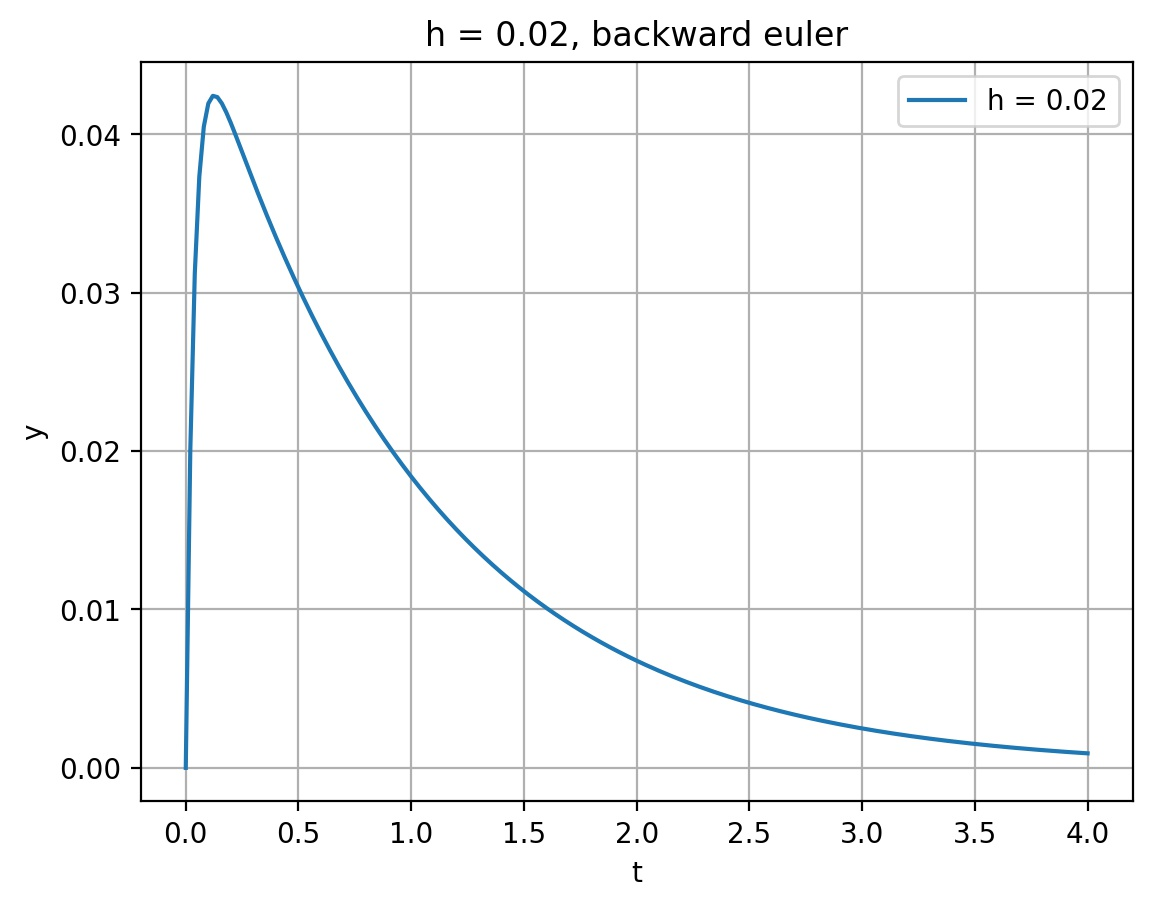
\includegraphics[width=.45\linewidth]{../p4/results/backward_euler_0.02.jpg}
		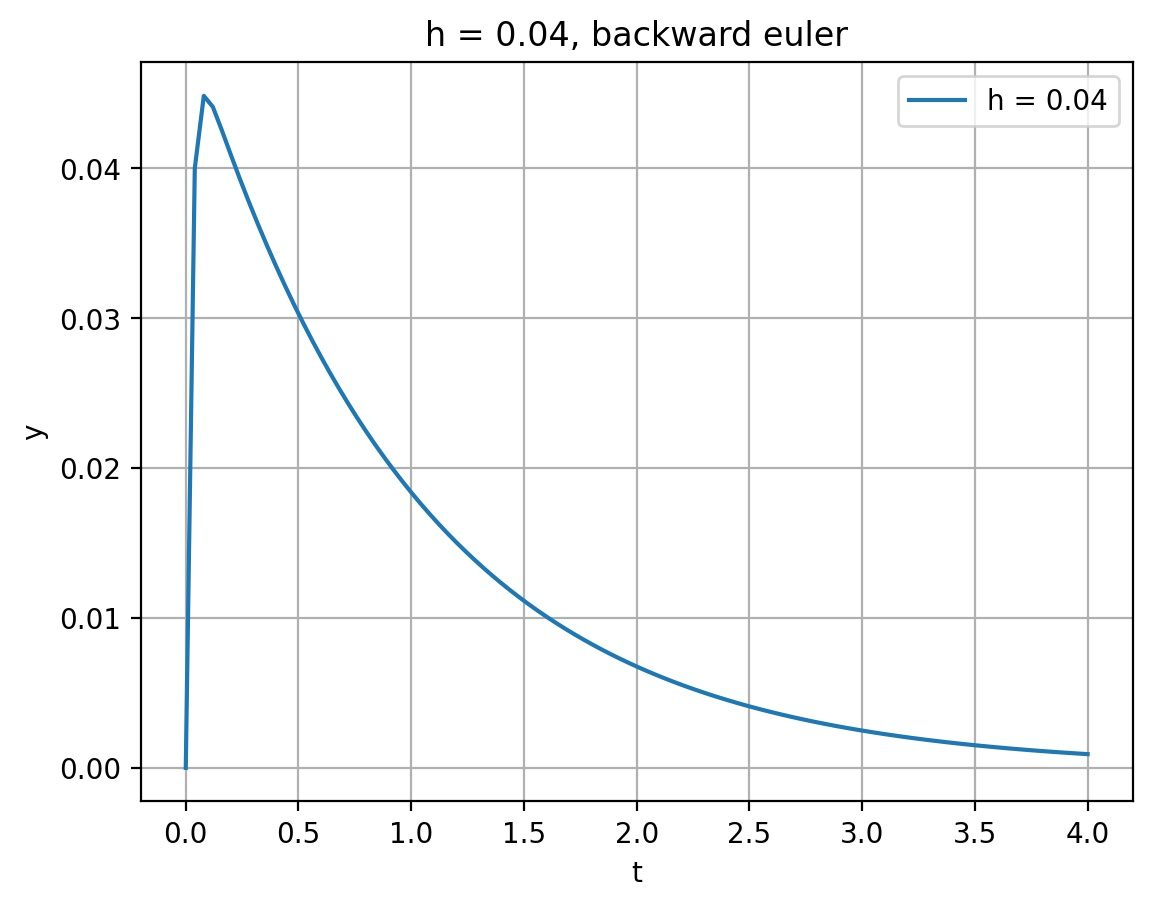
\includegraphics[width=.45\linewidth]{../p4/results/backward_euler_0.04.jpg}
		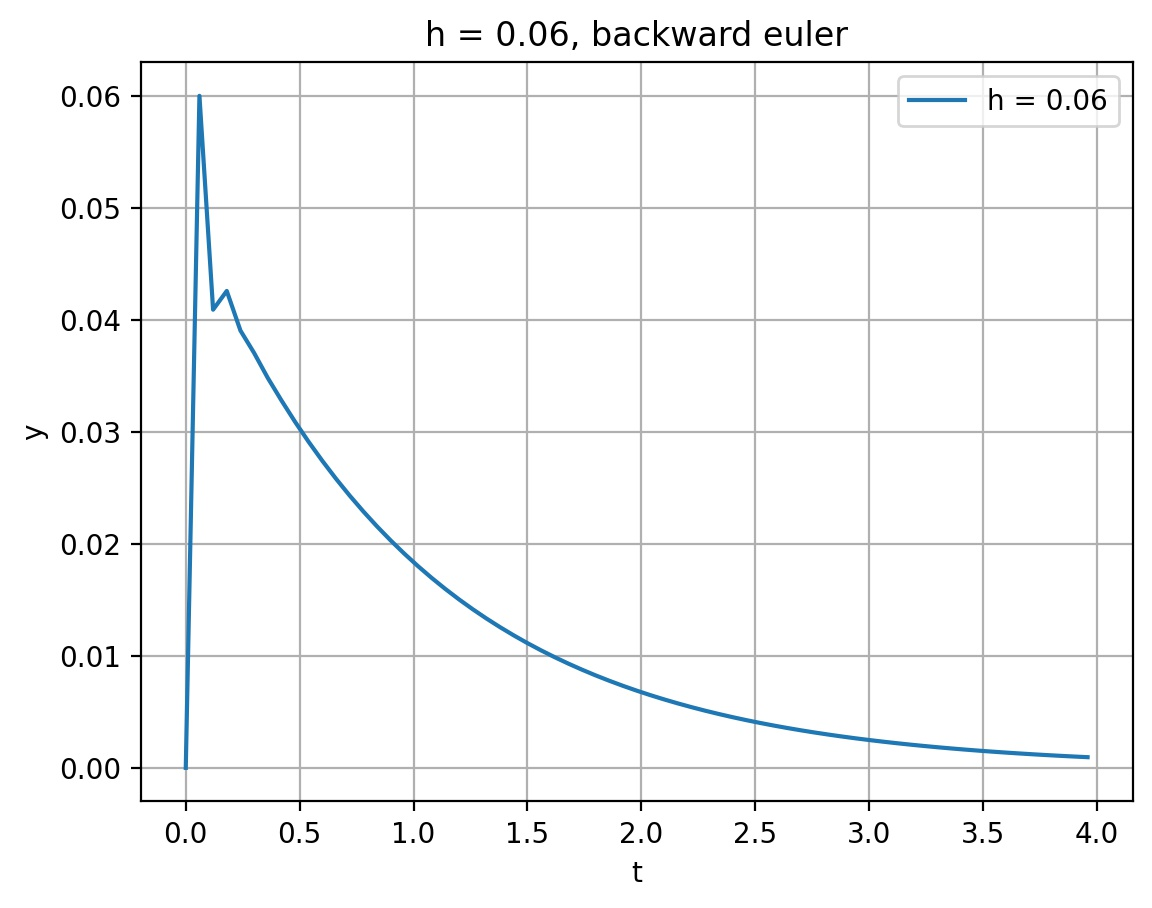
\includegraphics[width=.45\linewidth]{../p4/results/backward_euler_0.06.jpg}
		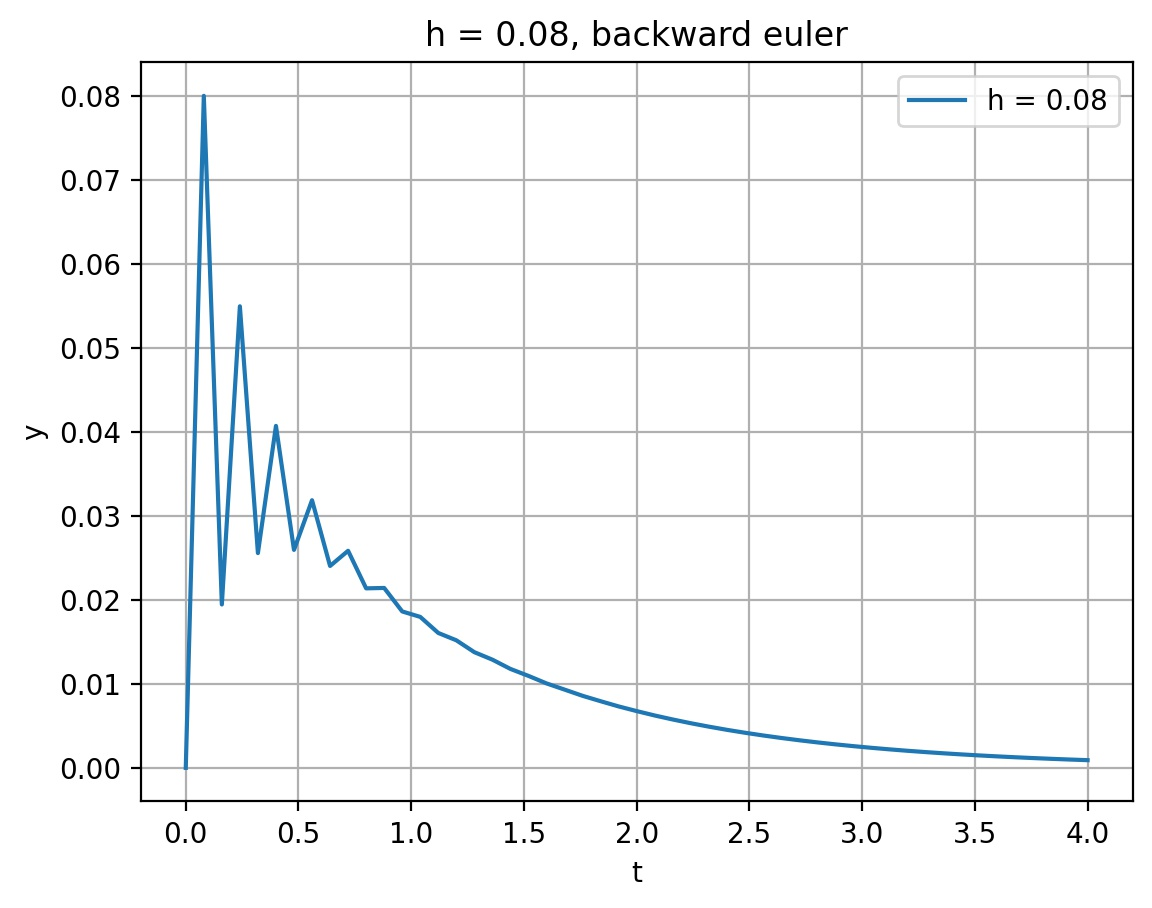
\includegraphics[width=.45\linewidth]{../p4/results/backward_euler_0.08.jpg}
		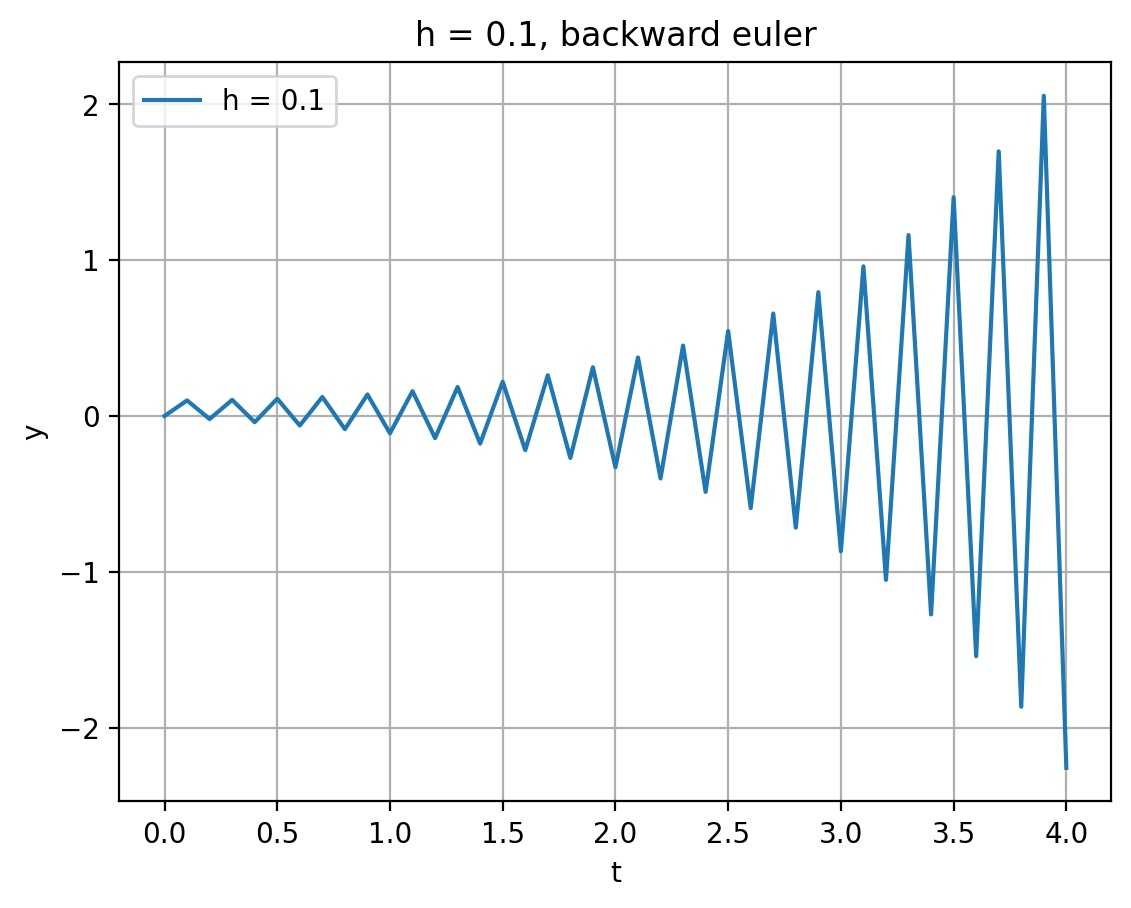
\includegraphics[width=.45\linewidth]{../p4/results/backward_euler_0.1.jpg}
		\caption{The integral curve for various values of $h$ using the backward euler method. It can be seen that from a value of $h$, the results 
			become \emph{unstable}}
		\label{fig:backward_euler}
	\end{figure}

	\subsection{Part C}
	The analytic result of the integral is:
	\begin{equation}
		y = \frac{1}{20} \left(e^{-t} - e^{-21t}\right)
	\end{equation}
	Since the algorithms take the
	count and the ending time for them isn't exactly $4$, in order to find the right value for error, I calculate the error by taking the real value for the 
	last time of each algorithm, and substract \emph{that} from the resulted value of that algorithm.

	You can see the values of runtime and error for each value of $h$ and for euler and backward euler in Table~\ref{tab:eulers}
	
	\begin{table}[h!]
		\centering
		\begin{tabular}{|c|c|c|c|c|}
\hline
 & \multicolumn{2}{|c|}{euler} & \multicolumn{2}{|c|}{backward euler}\\
\hline
h & runtime & error & runtime & error\\
 \hline
$0.01$ & $0.001356363$ & $-6.81 \times 10 ^{-7}$ & $0.00118112$ & $-2.28\times 10^{-7}$  \\
 \hline
$0.02$ & $0.000642061$ & $-1.35\times 10 ^{-6}$ & $0.00055789$ & $-4.54 \times 10^{-7}$ \\
 \hline
$0.04$ & $0.000321388$ & $-9.26 \times 10 ^{-6}$ & $0.00028133$ & $-9.028 \times 10^{-7}$ \\
 \hline
$0.06$ & $0.000210523$ & $-3.227$ & $0.00018715$ & $-1.399 \times 10^{-6}$ \\
 \hline
$0.08$ &$0.000161647$ & $29622$  & $0.00014257$ & $-1.78 \times 10^{-6}$ \\
 \hline
$0.1$ &$0.000129699$  & $-169639$ & $0.00011444$ & $-2.2575$ \\
\hline
		\end{tabular}
	\caption{data for euler and backward euler. As one can see, the backward euler method gives much more accurate results while the runtime 
	is almost the same.}
	\label{tab:eulers}
	\end{table}

	\subsection{Part D}
	I used the the following algorithm:
	\begin{equation}
		\begin{aligned}
			k &= \dot{y}(y_n, t) h\\
			\dot{y}_{n+1} &= \dot{y}(y_n + k, t + \frac{h}{2}) \\
			y_{n+1} &= y_n + \frac{\dot{y}_{n + 1} + \dot{y}_n}{2}  h\\
			\dot{y}_{n+1} &= \dot{y}(y_{n+1}, t + h) 
		\end{aligned}
	\end{equation}

	The values for runtime and error are in Table~\ref{tab:my_method}
	
		\begin{table}[h!]
		\centering
		\begin{tabular}{|c|c|c|}
			\hline
			h & runtime & error \\
			\hline
			$0.01$ & $0.002925872$ & $2.579 \times 10 ^{-6}$ \\
			\hline
			$0.02$ & $0.001465082$ & $5.903 \times 10 ^{-6}$ \\
			\hline
			$0.04$ & $0.000742435$ & $1.653 \times 10 ^{-5}$ \\
			\hline
			$0.06$ & $0.000485897$ & $4.276 \times 10 ^{-5}$  \\
			\hline
			$0.08$ &$0.000373840$ & $0.000156$  \\
			\hline
			$0.1$ &$0.000296592$  & $-2.01672$  \\
			\hline
		\end{tabular}
		\caption{data for \texttt{my\_method}. As one can see, my method gives accurate and more stable results that the euler method, while the 
			runtime is about 10 times that of euler.}
		\label{tab:my_method}
	\end{table}

	\section{Problem 5}
	I made a \texttt{System} class that takes the values for \texttt{r}, and makes the system. the \texttt{system\_play()} method randomly 
	matches the players into pairs. Then, these pairs play with each other and if their strategies differ, they both change their strategy for the next
	step. The \texttt{next\_step()} method plays the system for one step and updates the value of $Q$. Note that in \texttt{\_\_init\_\_()}, 
	\texttt{r} players have fixed strategies.
	\subsection{Part A}
	Here I plot the values for Q and the strategy of player 50 in the system. (Fig~\ref{fig:r_zero})
	
	\begin{figure}[h!]
		\centering
		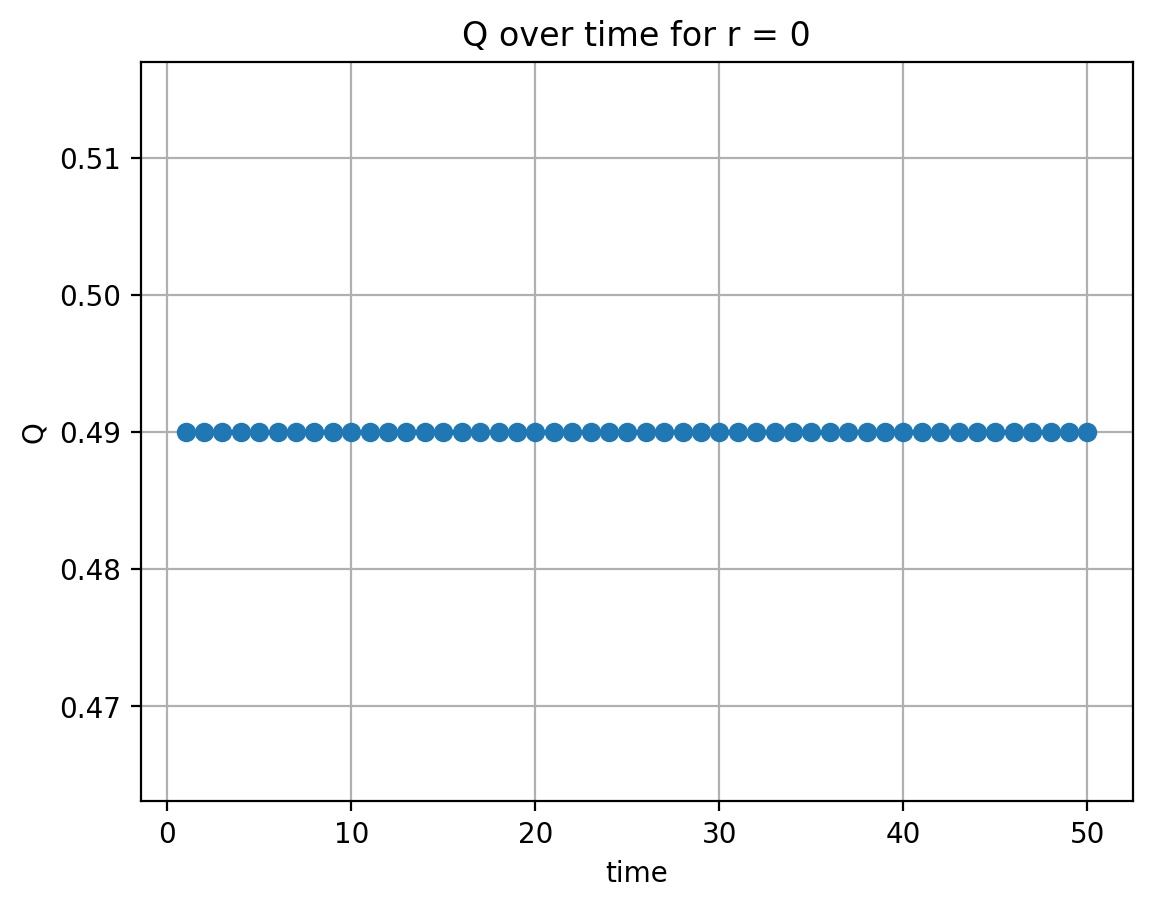
\includegraphics[width=.45\linewidth]{../p5/results/Q.jpg}
		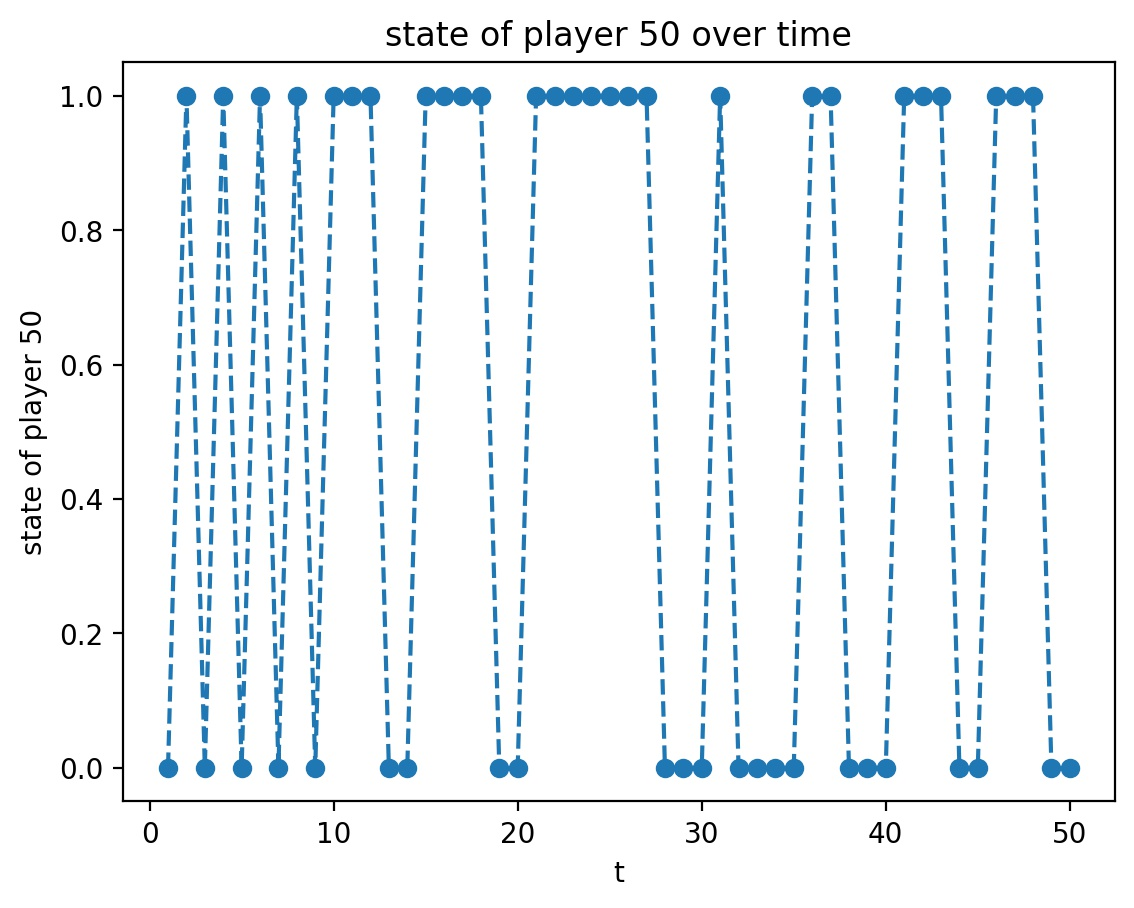
\includegraphics[width=.45\linewidth]{../p5/results/state50.jpg}
		\caption{As one  can see the system is dynamic and the states changes but the value for Q is fixed. This is due to the dynamic of the players,
		since if their strategies differ, they \emph{both} change strategy results in no change in Q}
		\label{fig:r_zero}
	\end{figure}
	
	\subsection{Part B}
	Here I plot the values of Q for the systems with \texttt{r} fixed players, varied from 0 to 10 for 50 time steps. (Fig~\ref{fig:Q})
	
	\begin{figure}[h!]
		\centering
		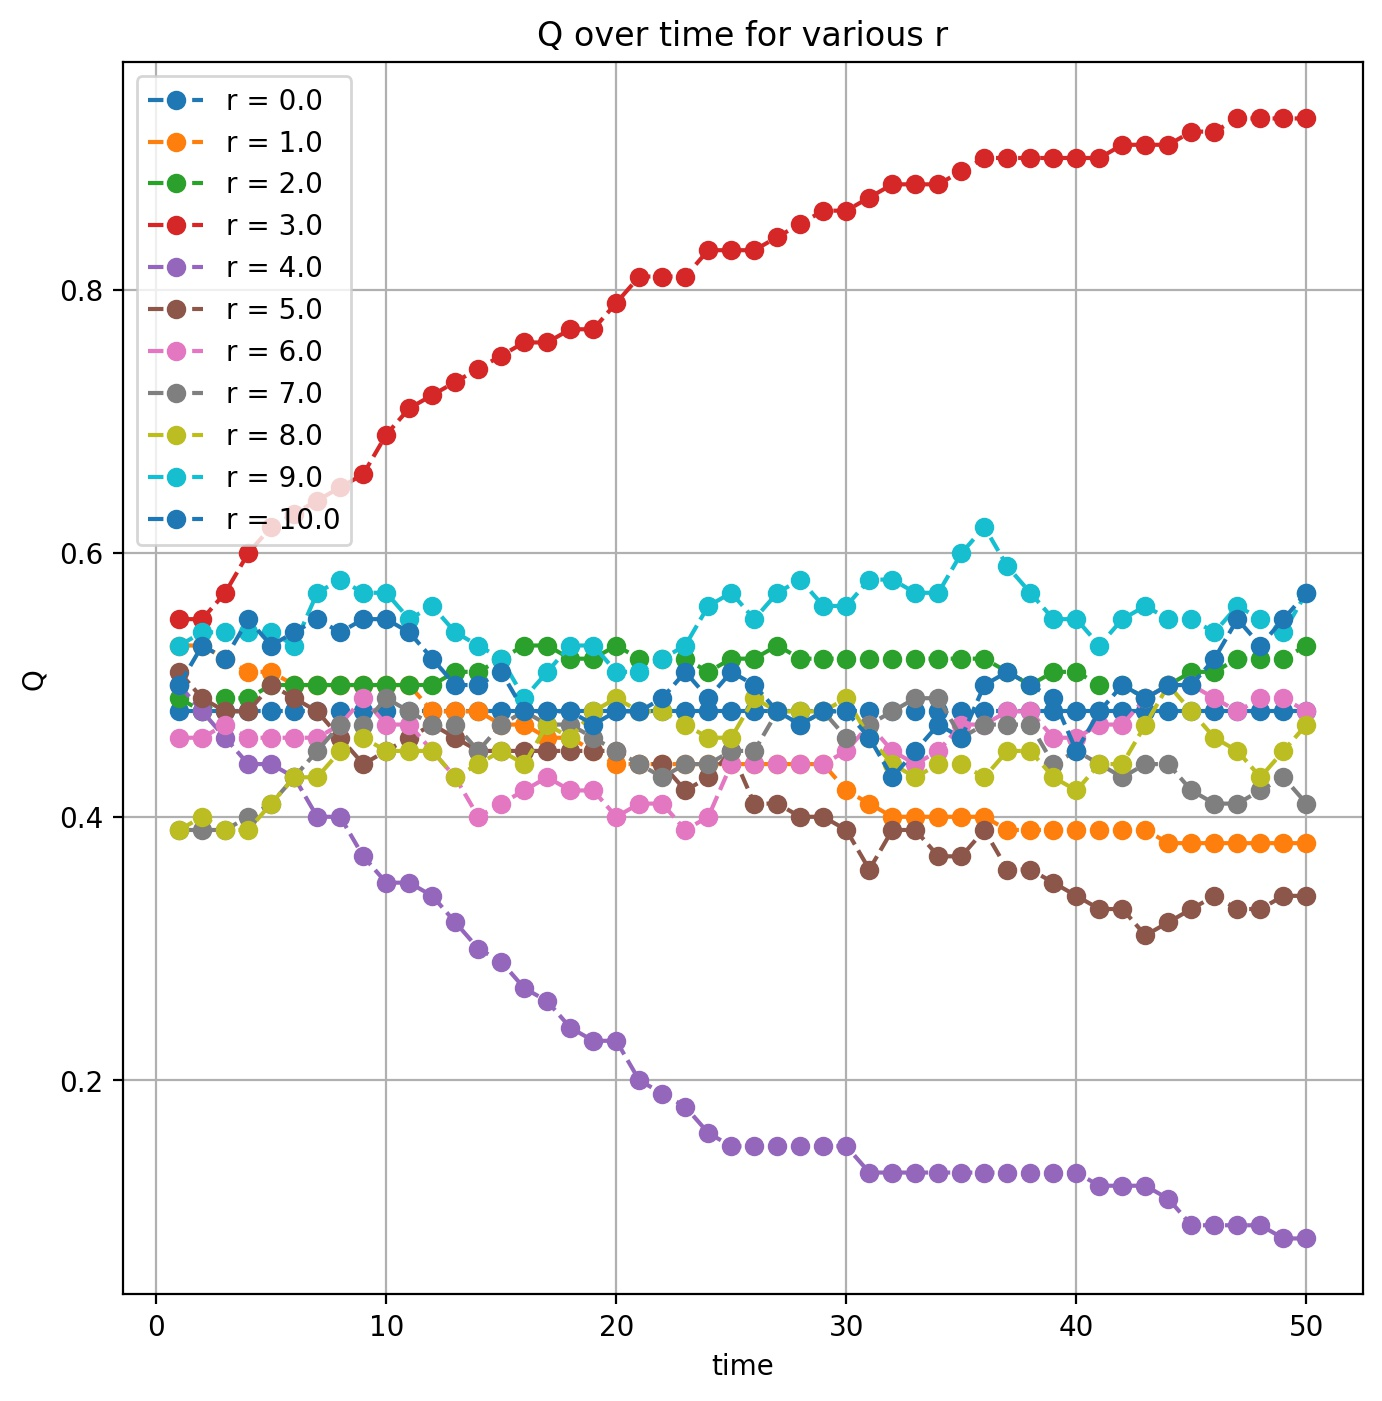
\includegraphics[width=0.9\linewidth]{../p5/results/Q_r.jpg}
		\caption{Now since some of the players are fixated on their strategies, $Q$ varies with time. We see that for intermediate values of r, 
		the system is divergent.}
		\label{fig:Q}
	\end{figure}

\end{document}